\chapter{Results and Discussion}
This chapter presents the results of training the Explainable Boosting Machine (EBM) on the extracted linguistic
features from the I-JAS corpus. The section begins with an overview of the model's performance, followed by an
analysis of feature importance and concludes with a discussion of the results in light of previous findings and
methodological considerations.


\section{Model Performance}
%*Discuss f1, accuracy, precision
%*share confusion matrix
%*discuss small sample size for N1 group which likely affected the classification
%*could not achieve better than 50\% accuracy, probably due to the 5 groups and overlap between some proficiency
%levels. Still better performance than the 20\% random guess baseline....

The EBM was trained using the full set of extracted features on a five-class classification task corresponding to
the five JLPT proficiency levels (N5-N1). The model was evaluated using 5 fold cross validation, with over sampling
used to balance the minority classes (N1). The results, aggregated across all cross validation folds, are summarized
in Table~
\ref{tab:trainingResults}.

%ToDO Update with correct values (I ran so many times need to confirm everything is the final version)
\begin{table}[h!]
    \centering
    \begin{tabular}{lcccc}
        \hline \textbf{Class} & \textbf{Precision} & \textbf{Recall} & \textbf{f1-score} & \textbf{Support} \\ \hline
        N5    &   0.46   &   0.51   &   0.48   &    735\\
          N4    &   0.44   &   0.41   &   0.43   &   1431\\
          N3    &   0.39   &   0.35   &   0.37  &    1342\\
          N2  &     0.34   &   0.39  &    0.36   &    816\\
          N1    &   0.14   &   0.17   &   0.16    &   224\\ \hline
        accuracy &   -    &      -    &     0.39  &    4548\\
   macro avg  &     0.36   &   0.37  &    0.36   &   4548\\
weighted avg  &     0.40  &    0.39    &  0.39   &   4548\\ \hline
    \end{tabular}
    \caption[Overall Classification Report (All Folds Combined)]{}
    \label{tab:trainingResults}
\end{table}

The model achieved an overall accuracy of 39\%, demonstrating some capacity to distinguish between proficiency
levels.
While the overall performance did not exceed 50\%, it represents a significant improvement over a random guess
baseline of 20\% for a five-class classification problem. The F1-scores, which provide a harmonic mean of precision
and recall ranged from .16 for N1 and .48 for N5 (Table~\ref{tab:trainingResults}).

Notably, classification performance declined as proficiency increased, with the N1 group showing the weakest
performance across all metrics (precision = 0.14, recall=0.17, f1=0.16). This is likely attributable in part to the
small sample size of N1 texts in the corpus, as well as the overlap between the proficiency levels.

Performance was highest for the N5 and N4 levels, which may reflect the chosen features may be more robust against
distinguishing the lower proficiency and intermediate levels. In contrast, the model struggled to differentiate
adjacent intermediate levels N3-N2, which suggests a need for more sensitive or diversified features as shown in the
confusion matrix in Figure~\ref{fig:conMA}.

\begin{figure}[h!]
           \centering
           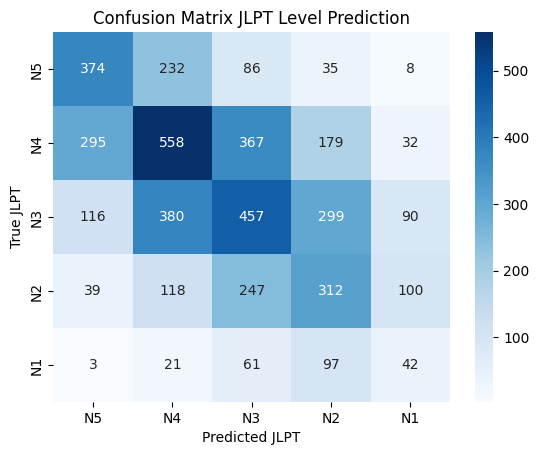
\includegraphics[scale=.4]{img/confusionMatrix}
           \caption[Confusion Matrix for JLPT Level Prediction]{}
           \label{fig:conMA}
\end{figure}

A common mis-classification was a substantial number of true N3 instances were misclassified as N4(368) or N2 (306).
Similarly, N2 texts were frequently predicted as N3(245) or N1 (107), and N1 texts were often misclassified as N2(
98) or N3(62). This suggests that the model frequently confused text belonging to adjacent proficiency levels,
indicating a high overlap between the proficiency levels. This was confirmed when

When aggregating the proficiency levels into 3 groups - Beginner (N5+N4), Intermediate (N3+N2), and Advanced (N1)
Classification of the three groups improved greatly (), supporting the fact that there exists overlap between the
proficiency levels making it difficult for the model to distinguish between adjacent classes.

\section{Feature Importance Analysis}
\begin{figure}[h!]
    \centering
    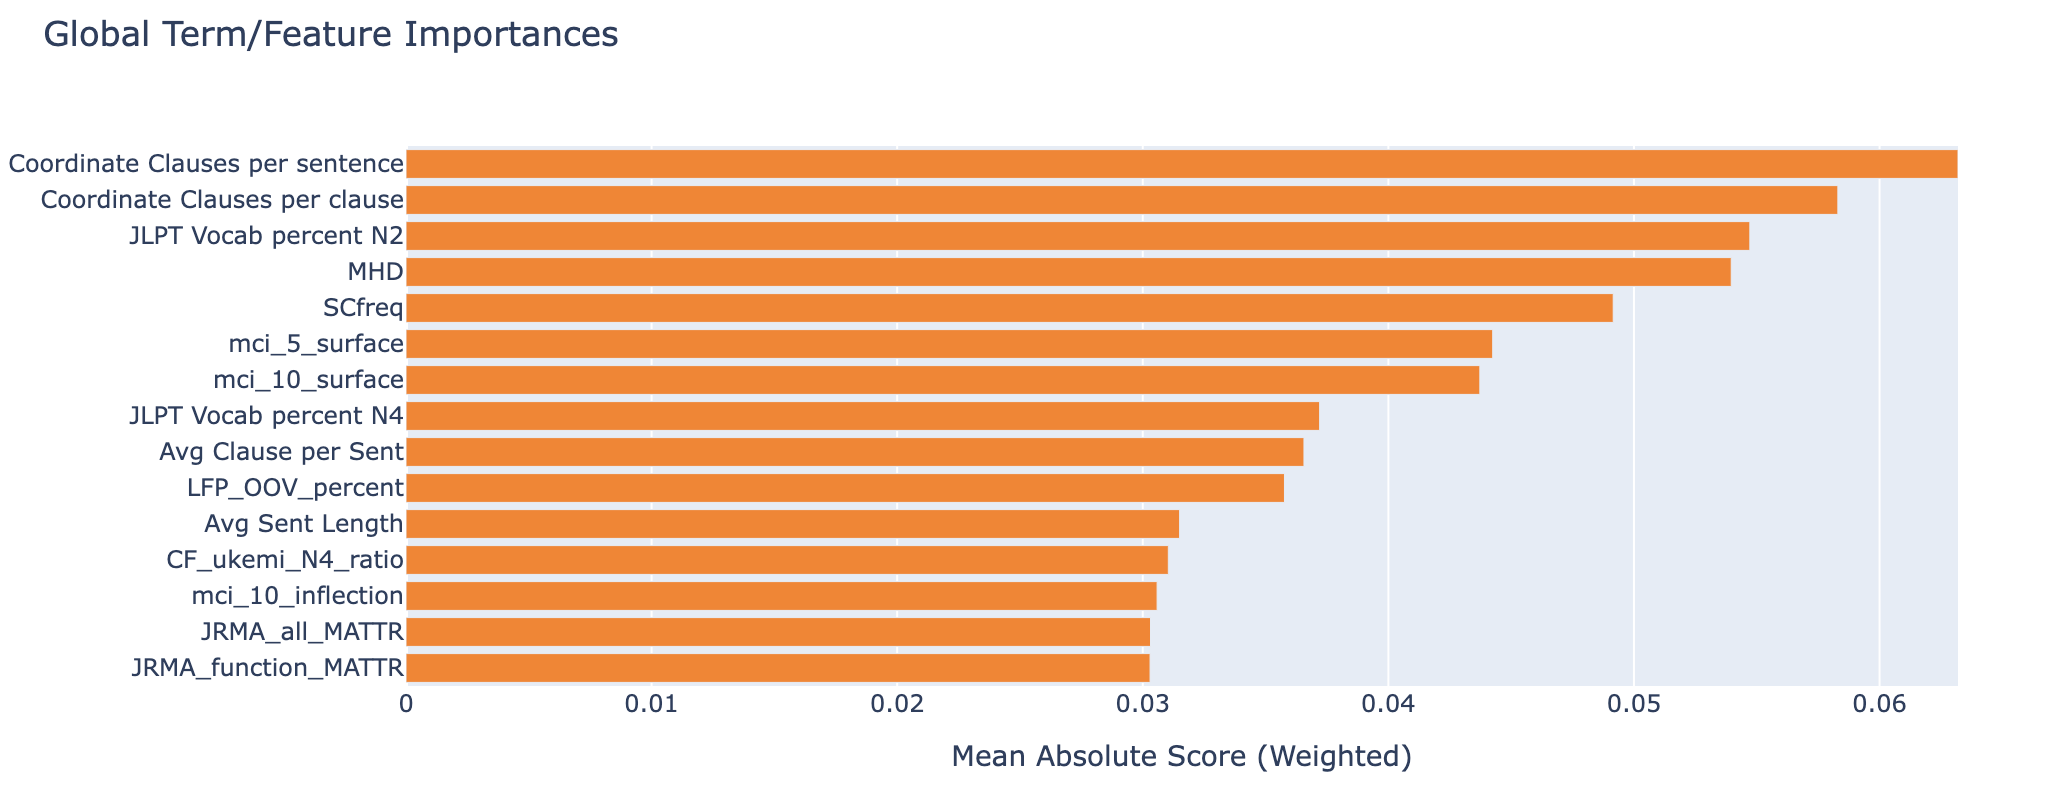
\includegraphics[scale=.4]{img/feature_importance}
    \caption[Feature Importance Chart]{The chart of features contributing to the classificaiton of JLPT proficency levels and their weighted
    scores.}
    \label{fig:featureimportance}
\end{figure}

Mostly complexity measures were seen as the important features in the top 15 however a diverse variety of complexity
measures are used from Syntactic Complexity Measures, lexical sophistication, morphological

Coordinate Clauses per sentence and Coordinate Clauses per clause : were the two top contributing features

Percent of N2 vocabulary :

Scfreq: This distinguished from the lower proficiency levels, here it is ranked as the 5th strongest feature
contributing to classification. Which surprised me as this feature uses subordinating conjunctions as a proxy to
measure subordination.

Ukemi - passive form was the only criterial feature in top 15.


\section{Discussion}

% Make conrete citations
The results above provide partial support for developmental patterns identified in the previous chapters. In
particular, some features showed a clear trajectory of increased usage of complexity across levels, supporting
earlier corpus based findings and previous literature. However the predictive power of many features was moderate,
as found in the f1 scores, and some expected distinctions between adjacent levels (e.g. N3 vs N2) were not captured
effectively.

This suggest that while form-based measures of grammatical complexity and frequency based criterial features can be
useful, they may not be sufficienct in isolation. Some grammatical forms exhibit nuanced usage that depends on
semantic, pracmatic, or discourse-level factors- dimensions that are not easily captured through surface-form
analysis alone.

The model's diminished performance, particularly for N2 and N1 as evidenced by lower f1-scores and the high number
of misclassifications in the confusion matrix (Figure~\ref{fig:conMA}), points to inherent challenges in
classifying these adjacent proficiency levels. The significant overlap observed in predictions (e.g. N3 misclassified
as N2 and N4) suggests that the linguistic differences between intermediate and advanced levels are subtler and less
discretely based on the current feature set. It is plausible after all, that learners at adjacent intermediate
levels exhibit similar linguistic characteristics than, for example, a beginner (N5) and an advanced learner (N1).
This continuous nature of language development makes sharp categorical distinctions difficult for any model.

%ToDO get total number of texts written from N1 level
The small sample size of N1 group (44 participants, ) significantly impacted its classification accuracy (F1-score
of 0.17 in Table~\ref{tab:trainingResults}). With fewer examples, the model had limited data to learn the specific
criteria that distinguish N1 texts from other levels, leading to a high rate of misclassification, particularly into
N2 and N3 categories. This data imbalance likely constrained the model's ability to fully capture the
characteristics of advanced learners.




\subsection{Limitations and Difficulties}
The corpus, consisting of uncorrected learner language, posed challenges for feature extraction. Misspellings and
grammatical errors common in learner output could lead to incorrect tokenization and POS tagging by the underlying
NLP tools (e.g. SpaCy's Ginza package), thus impacting the accuracy of extracted features. For instance, irregular
forms of "mispellings" might be incorrectly counted as out-of-vocabulary words (in the context of the LFP complexity
measure), rather than as specific error types. More crucially, the morphological complexity of Japanese,
particularly with compound verbs and auxiliary constructions (e.g. 「言い切る」 as one verb vs. 「食べ切る」 parsed into two
parts), meant that rule-based feature extraction struggled with consistency. This could lead to undercounting or
miscategorizing certain complex forms, which are critical indicators of advanced proficiency.

The variability in text length, with some text being very short, likely affected the reliability of certain
density-based metrics, such as MTLD (Mean Type-Token Ratio), if it were included. Such metrics are sensitive to text
length, and calculation over very short texts can yield less stable or representative values, potentially
introducing noise into the feature set.

While features like coordinate clauses per sentence were highly important, the accuracy of their extraction was
dependent on the underlying tokenizer's ability to correctly identify conjunctions and clause boundaries. As noted
previously, many Japanese conjunctions can be used in both coordinating and subordinating contexts, and rule-based
parsers like SpacCy may not fully account for contextual nuances. This potential inaccuracy in the input features
could directly limit the model's ability to use these syntactic measures for precise classification. A more robust,
context-aware parsing system would likely improve the quality of these features.



shortfalls/difficulties
- mention lerner language and the corpus being uncorrected so this may lead to misinterpretations by the tokenizer to classify things correctly.
    also difficulties in capturing lexical forms - many "mispellings" included on LFP OOV list.
- issue of some texts being too short for MTLD calculation
- use of only form-based grammar difficulty in correctly extracting meaning based forms
- also difficulty of not knowing which forms are considered one word expressions versus expressions that will
actually be broken down into smaller parts by the tokenizer (as noted below with 言い切る etc.) meaning not all forms
will be extracted
-small N1 group size effecting model training, and also the statistical relavance of certain features.
-Possible overlap between adjacent levels making it difficult to correctly predict....

In consistency in parsing of 〜切るto show completely finishing an action. 言い切る 売り切る are considered one verb. in the
case of 食べ(verb) 切る(非自立可能Verb) and 食べ(Verb) 切れる (AUX 非自立可能) makes it difficult to when dealing with rule based
matching to extract the form..死ぬほど and other constructions with ほどare also similar.

-Issues with clause parsing - the tokenizer by spacy is inaccurate in classyfying some coordinating and
subordinating conjunctions - many conjunctions in Japanese can be used in both contexts and spacy doesn't take the
context into consideration when labeling the conjunctions. - tried to mitigate this by using a rule based formula to
classify coordinating and subordinating clauses but it is difficult to control for each case. thereofore a more
robust system would possibly lead to better results......I need to say something more about clausal use in Japanese
for learners.


Need to mention the feature extractor follows rules for the standardized language which is widely taught to
learners. Variations due to dialects and casual written variations not included and therefore this would not be
able to extract text with these. Also chose grammar constructs which were largely form based (i.e. easier to extract
vs. use based) and ones that are likely to be used in written language. (leaving out spoken expressions as they
wouldn't likely appear much in writing. )

Mention again the shortfall of not analyzing errors or having them as a feature, this could probably lead to better
classification

Also the fact that these JLPT levels are approximated from J-Cat - although they have been validated, JLPT does not
cover writing or speaking (production) so there can be large variance in what someone who passes one of the JLPT
tests can actually accomplish with the language.